\begin{figure}[!htbp]
\begin{center}
\begin{tikzpicture}[scale=0.8, transform shape]
    %\draw [help lines] (0, 0) grid (10, 7);
    \draw (0, 0) node {\begin{tikzpicture}[scale=1.0, transform shape]
    \node[draw=white, thick] (puRadio) {
        \begin{tikzpicture} [scale=0.5]
        \draw [line width=0.25mm, bend right = 15, red] (2, -0.44) to (2.5,0.44);
        \draw [line width=0.25mm, bend left = 15, red] (3, -0.44) to (2.5,0.44);
        \draw [line width=0.25mm, red] (2.15, -0.3) to (2.85,-0.3);
        \draw [line width=0.25mm, red] (2.25, -0.15) to (2.75,-0.15);
        \draw [line width=0.25mm, red] (2.35, 0) to (2.65,0);
        %\draw [line width=0.25mm] (2.5, -0.44) to (2.5,0.44);
        \draw [fill=red, red] (2.5,0.44) circle(1.5mm);

        \draw [line width=0.25mm, red] (2.5, 0.725) to (2.5,1.0);
        \draw [line width=0.25mm, red] (2.65, 0.65) to (2.825,0.85);
        \draw [line width=0.25mm, red] (2.725, 0.44) to (3,0.44);
        \draw [line width=0.25mm, red] (2.35, 0.65) to (2.175,0.85);
        \draw [line width=0.25mm, red] (2.275, 0.44) to (2,0.44);

        \end{tikzpicture}
    };
\end{tikzpicture}};
    \draw (0, 7) node {\begin{tikzpicture}[scale=1.0, transform shape]
    \node[draw=white, thick] (puRadio) {
        \begin{tikzpicture} [scale=0.5]
        \draw [line width=0.25mm, bend right = 15, red] (2, -0.44) to (2.5,0.44);
        \draw [line width=0.25mm, bend left = 15, red] (3, -0.44) to (2.5,0.44);
        \draw [line width=0.25mm, red] (2.15, -0.3) to (2.85,-0.3);
        \draw [line width=0.25mm, red] (2.25, -0.15) to (2.75,-0.15);
        \draw [line width=0.25mm, red] (2.35, 0) to (2.65,0);
        %\draw [line width=0.25mm] (2.5, -0.44) to (2.5,0.44);
        \draw [fill=red, red] (2.5,0.44) circle(1.5mm);

        \draw [line width=0.25mm, red] (2.5, 0.725) to (2.5,1.0);
        \draw [line width=0.25mm, red] (2.65, 0.65) to (2.825,0.85);
        \draw [line width=0.25mm, red] (2.725, 0.44) to (3,0.44);
        \draw [line width=0.25mm, red] (2.35, 0.65) to (2.175,0.85);
        \draw [line width=0.25mm, red] (2.275, 0.44) to (2,0.44);

        \end{tikzpicture}
    };
\end{tikzpicture}};
    \draw (10, 7) node {\begin{tikzpicture}[scale=1.0, transform shape]
    \node[draw=white, thick] (puRadio) {
        \begin{tikzpicture} [scale=0.5]
        \draw [line width=0.25mm, bend right = 15, red] (2, -0.44) to (2.5,0.44);
        \draw [line width=0.25mm, bend left = 15, red] (3, -0.44) to (2.5,0.44);
        \draw [line width=0.25mm, red] (2.15, -0.3) to (2.85,-0.3);
        \draw [line width=0.25mm, red] (2.25, -0.15) to (2.75,-0.15);
        \draw [line width=0.25mm, red] (2.35, 0) to (2.65,0);
        %\draw [line width=0.25mm] (2.5, -0.44) to (2.5,0.44);
        \draw [fill=red, red] (2.5,0.44) circle(1.5mm);

        \draw [line width=0.25mm, red] (2.5, 0.725) to (2.5,1.0);
        \draw [line width=0.25mm, red] (2.65, 0.65) to (2.825,0.85);
        \draw [line width=0.25mm, red] (2.725, 0.44) to (3,0.44);
        \draw [line width=0.25mm, red] (2.35, 0.65) to (2.175,0.85);
        \draw [line width=0.25mm, red] (2.275, 0.44) to (2,0.44);

        \end{tikzpicture}
    };
\end{tikzpicture}};
    \draw (10, 0) node {\begin{tikzpicture}[scale=1.0, transform shape]
    \node[draw=white, thick] (puRadio) {
        \begin{tikzpicture} [scale=0.5]
        \draw [line width=0.25mm, bend right = 15, red] (2, -0.44) to (2.5,0.44);
        \draw [line width=0.25mm, bend left = 15, red] (3, -0.44) to (2.5,0.44);
        \draw [line width=0.25mm, red] (2.15, -0.3) to (2.85,-0.3);
        \draw [line width=0.25mm, red] (2.25, -0.15) to (2.75,-0.15);
        \draw [line width=0.25mm, red] (2.35, 0) to (2.65,0);
        %\draw [line width=0.25mm] (2.5, -0.44) to (2.5,0.44);
        \draw [fill=red, red] (2.5,0.44) circle(1.5mm);

        \draw [line width=0.25mm, red] (2.5, 0.725) to (2.5,1.0);
        \draw [line width=0.25mm, red] (2.65, 0.65) to (2.825,0.85);
        \draw [line width=0.25mm, red] (2.725, 0.44) to (3,0.44);
        \draw [line width=0.25mm, red] (2.35, 0.65) to (2.175,0.85);
        \draw [line width=0.25mm, red] (2.275, 0.44) to (2,0.44);

        \end{tikzpicture}
    };
\end{tikzpicture}};
    %\draw [fill=green!50!white] (-2, -2) rectangle (2, -1);
    
    \pause
    
    \draw (5, 4.9) node {
\begin{tikzpicture}[scale=1.0, transform shape]
    \tikzstyle{every node} = [draw, shape = rectangle, node distance=0mm, minimum width=4mm, minimum height=6mm, fill=green!25!white]
    \node[draw=black, thick, minimum width=25mm] (channel1) {};
\end{tikzpicture}
};
    \draw (5, 4.2) node {
\begin{tikzpicture}[scale=1.0, transform shape]
    \tikzstyle{every node} = [draw, shape = rectangle, node distance=0mm, minimum width=4mm, minimum height=6mm, fill=green!25!white]
    \node[draw=black, thick, minimum width=25mm] (channel1) {};
\end{tikzpicture}
};
    \draw (5, 3.5) node {
\begin{tikzpicture}[scale=1.0, transform shape]
    \tikzstyle{every node} = [draw, shape = rectangle, node distance=0mm, minimum width=4mm, minimum height=6mm, fill=green!25!white]
    \node[draw=black, thick, minimum width=25mm] (channel1) {};
\end{tikzpicture}
};
    \draw (5, 2.8) node {
\begin{tikzpicture}[scale=1.0, transform shape]
    \tikzstyle{every node} = [draw, shape = rectangle, node distance=0mm, minimum width=4mm, minimum height=6mm, fill=green!25!white]
    \node[draw=black, thick, minimum width=25mm] (channel1) {};
\end{tikzpicture}
}; % [label=below:{\tiny \(n\) spectrum channels}]
    
    \pause
    
    \draw (5, 6.2) node {\begin{tikzpicture}[scale=0.375, transform shape]
    \node (controlRadio)
    {
        \begin{tikzpicture} [scale=1.0]
        \draw [fill=blue!25!white, blue!75!black] (2.3, -0.44) -- (2.5,0.44) -- (2.7, -0.44);
        \draw [fill=blue!25!white, blue!75!black] (2.5,0.44) circle(1.5mm);

        \draw [line width=0.25mm, blue!25!white] (2.5, 0.725) to (2.5,1.0);
        \draw [line width=0.25mm, blue!25!white] (2.65, 0.65) to (2.825,0.85);
        \draw [line width=0.25mm, blue!25!white] (2.725, 0.44) to (3,0.44);
        \draw [line width=0.25mm, blue!25!white] (2.35, 0.65) to (2.175,0.85);
        \draw [line width=0.25mm, blue!25!white] (2.275, 0.44) to (2,0.44);

        \end{tikzpicture}
    };
    \node (dataRadio1) [below=of controlRadio, xshift=-1.0cm, yshift=0.5cm] %, xshift=-1.5mm
    {
        
\begin{tikzpicture} [scale=0.75]
        \draw [line width=0.25mm, green!50!black] (2, -0.44) to (2.5,0.44);
        \draw [line width=0.25mm, green!50!black] (3, -0.44) to (2.5,0.44);
        \draw [line width=0.25mm, green!50!black] (2, -0.44) to (3,-0.44);
        \draw [line width=0.25mm, green!50!black] (2.5, -0.44) to (2.5,0.44);
        \draw [fill=green!50!black, green!50!black] (2.5,0.44) circle(1.5mm);

        \draw [line width=0.25mm, green!50!black] (2.5, 0.725) to (2.5,1.0);
        \draw [line width=0.25mm, green!50!black] (2.65, 0.65) to (2.825,0.85);
        \draw [line width=0.25mm, green!50!black] (2.725, 0.44) to (3,0.44);
        \draw [line width=0.25mm, green!50!black] (2.35, 0.65) to (2.175,0.85);
        \draw [line width=0.25mm, green!50!black] (2.275, 0.44) to (2,0.44);

        \end{tikzpicture}
    };
    %()
    \draw[fill=green!50!black, green!50!black] (-0.25,-2.15) circle (0.025);
    \draw[fill=green!50!black, green!50!black] (0,-2.15) circle (0.025);
    \draw[fill=green!50!black, green!50!black] (0.25,-2.15) circle (0.025);
    %
    \node (dataRadio2) [right=of dataRadio1] %, xshift=-1.5mm
    {
        
\begin{tikzpicture} [scale=0.75]
        \draw [line width=0.25mm, green!50!black] (2, -0.44) to (2.5,0.44);
        \draw [line width=0.25mm, green!50!black] (3, -0.44) to (2.5,0.44);
        \draw [line width=0.25mm, green!50!black] (2, -0.44) to (3,-0.44);
        \draw [line width=0.25mm, green!50!black] (2.5, -0.44) to (2.5,0.44);
        \draw [fill=green!50!black, green!50!black] (2.5,0.44) circle(1.5mm);

        \draw [line width=0.25mm, green!50!black] (2.5, 0.725) to (2.5,1.0);
        \draw [line width=0.25mm, green!50!black] (2.65, 0.65) to (2.825,0.85);
        \draw [line width=0.25mm, green!50!black] (2.725, 0.44) to (3,0.44);
        \draw [line width=0.25mm, green!50!black] (2.35, 0.65) to (2.175,0.85);
        \draw [line width=0.25mm, green!50!black] (2.275, 0.44) to (2,0.44);

        \end{tikzpicture}
    };%fill=green!50!black,
    \draw[line width=0.25mm, green!25!black] (0.25,-1) circle (3);
\end{tikzpicture}
};
    \draw (1.5, 4) node {\begin{tikzpicture}[scale=0.375, transform shape]
    \node (controlRadio)
    {
        \begin{tikzpicture} [scale=1.0]
        \draw [fill=blue!25!white, blue!75!black] (2.3, -0.44) -- (2.5,0.44) -- (2.7, -0.44);
        \draw [fill=blue!25!white, blue!75!black] (2.5,0.44) circle(1.5mm);

        \draw [line width=0.25mm, blue!25!white] (2.5, 0.725) to (2.5,1.0);
        \draw [line width=0.25mm, blue!25!white] (2.65, 0.65) to (2.825,0.85);
        \draw [line width=0.25mm, blue!25!white] (2.725, 0.44) to (3,0.44);
        \draw [line width=0.25mm, blue!25!white] (2.35, 0.65) to (2.175,0.85);
        \draw [line width=0.25mm, blue!25!white] (2.275, 0.44) to (2,0.44);

        \end{tikzpicture}
    };
    \node (dataRadio1) [below=of controlRadio, xshift=-1.0cm, yshift=0.5cm] %, xshift=-1.5mm
    {
        
\begin{tikzpicture} [scale=0.75]
        \draw [line width=0.25mm, green!50!black] (2, -0.44) to (2.5,0.44);
        \draw [line width=0.25mm, green!50!black] (3, -0.44) to (2.5,0.44);
        \draw [line width=0.25mm, green!50!black] (2, -0.44) to (3,-0.44);
        \draw [line width=0.25mm, green!50!black] (2.5, -0.44) to (2.5,0.44);
        \draw [fill=green!50!black, green!50!black] (2.5,0.44) circle(1.5mm);

        \draw [line width=0.25mm, green!50!black] (2.5, 0.725) to (2.5,1.0);
        \draw [line width=0.25mm, green!50!black] (2.65, 0.65) to (2.825,0.85);
        \draw [line width=0.25mm, green!50!black] (2.725, 0.44) to (3,0.44);
        \draw [line width=0.25mm, green!50!black] (2.35, 0.65) to (2.175,0.85);
        \draw [line width=0.25mm, green!50!black] (2.275, 0.44) to (2,0.44);

        \end{tikzpicture}
    };
    %()
    \draw[fill=green!50!black, green!50!black] (-0.25,-2.15) circle (0.025);
    \draw[fill=green!50!black, green!50!black] (0,-2.15) circle (0.025);
    \draw[fill=green!50!black, green!50!black] (0.25,-2.15) circle (0.025);
    %
    \node (dataRadio2) [right=of dataRadio1] %, xshift=-1.5mm
    {
        
\begin{tikzpicture} [scale=0.75]
        \draw [line width=0.25mm, green!50!black] (2, -0.44) to (2.5,0.44);
        \draw [line width=0.25mm, green!50!black] (3, -0.44) to (2.5,0.44);
        \draw [line width=0.25mm, green!50!black] (2, -0.44) to (3,-0.44);
        \draw [line width=0.25mm, green!50!black] (2.5, -0.44) to (2.5,0.44);
        \draw [fill=green!50!black, green!50!black] (2.5,0.44) circle(1.5mm);

        \draw [line width=0.25mm, green!50!black] (2.5, 0.725) to (2.5,1.0);
        \draw [line width=0.25mm, green!50!black] (2.65, 0.65) to (2.825,0.85);
        \draw [line width=0.25mm, green!50!black] (2.725, 0.44) to (3,0.44);
        \draw [line width=0.25mm, green!50!black] (2.35, 0.65) to (2.175,0.85);
        \draw [line width=0.25mm, green!50!black] (2.275, 0.44) to (2,0.44);

        \end{tikzpicture}
    };%fill=green!50!black,
    \draw[line width=0.25mm, green!25!black] (0.25,-1) circle (3);
\end{tikzpicture}
};
    \draw (2.5, 1) node {\begin{tikzpicture}[scale=0.375, transform shape]
    \node (controlRadio)
    {
        \begin{tikzpicture} [scale=1.0]
        \draw [fill=blue!25!white, blue!75!black] (2.3, -0.44) -- (2.5,0.44) -- (2.7, -0.44);
        \draw [fill=blue!25!white, blue!75!black] (2.5,0.44) circle(1.5mm);

        \draw [line width=0.25mm, blue!25!white] (2.5, 0.725) to (2.5,1.0);
        \draw [line width=0.25mm, blue!25!white] (2.65, 0.65) to (2.825,0.85);
        \draw [line width=0.25mm, blue!25!white] (2.725, 0.44) to (3,0.44);
        \draw [line width=0.25mm, blue!25!white] (2.35, 0.65) to (2.175,0.85);
        \draw [line width=0.25mm, blue!25!white] (2.275, 0.44) to (2,0.44);

        \end{tikzpicture}
    };
    \node (dataRadio1) [below=of controlRadio, xshift=-1.0cm, yshift=0.5cm] %, xshift=-1.5mm
    {
        
\begin{tikzpicture} [scale=0.75]
        \draw [line width=0.25mm, green!50!black] (2, -0.44) to (2.5,0.44);
        \draw [line width=0.25mm, green!50!black] (3, -0.44) to (2.5,0.44);
        \draw [line width=0.25mm, green!50!black] (2, -0.44) to (3,-0.44);
        \draw [line width=0.25mm, green!50!black] (2.5, -0.44) to (2.5,0.44);
        \draw [fill=green!50!black, green!50!black] (2.5,0.44) circle(1.5mm);

        \draw [line width=0.25mm, green!50!black] (2.5, 0.725) to (2.5,1.0);
        \draw [line width=0.25mm, green!50!black] (2.65, 0.65) to (2.825,0.85);
        \draw [line width=0.25mm, green!50!black] (2.725, 0.44) to (3,0.44);
        \draw [line width=0.25mm, green!50!black] (2.35, 0.65) to (2.175,0.85);
        \draw [line width=0.25mm, green!50!black] (2.275, 0.44) to (2,0.44);

        \end{tikzpicture}
    };
    %()
    \draw[fill=green!50!black, green!50!black] (-0.25,-2.15) circle (0.025);
    \draw[fill=green!50!black, green!50!black] (0,-2.15) circle (0.025);
    \draw[fill=green!50!black, green!50!black] (0.25,-2.15) circle (0.025);
    %
    \node (dataRadio2) [right=of dataRadio1] %, xshift=-1.5mm
    {
        
\begin{tikzpicture} [scale=0.75]
        \draw [line width=0.25mm, green!50!black] (2, -0.44) to (2.5,0.44);
        \draw [line width=0.25mm, green!50!black] (3, -0.44) to (2.5,0.44);
        \draw [line width=0.25mm, green!50!black] (2, -0.44) to (3,-0.44);
        \draw [line width=0.25mm, green!50!black] (2.5, -0.44) to (2.5,0.44);
        \draw [fill=green!50!black, green!50!black] (2.5,0.44) circle(1.5mm);

        \draw [line width=0.25mm, green!50!black] (2.5, 0.725) to (2.5,1.0);
        \draw [line width=0.25mm, green!50!black] (2.65, 0.65) to (2.825,0.85);
        \draw [line width=0.25mm, green!50!black] (2.725, 0.44) to (3,0.44);
        \draw [line width=0.25mm, green!50!black] (2.35, 0.65) to (2.175,0.85);
        \draw [line width=0.25mm, green!50!black] (2.275, 0.44) to (2,0.44);

        \end{tikzpicture}
    };%fill=green!50!black,
    \draw[line width=0.25mm, green!25!black] (0.25,-1) circle (3);
\end{tikzpicture}
};
    \draw (7.5, 1) node {\begin{tikzpicture}[scale=0.375, transform shape]
    \node (controlRadio)
    {
        \begin{tikzpicture} [scale=1.0]
        \draw [fill=blue!25!white, blue!75!black] (2.3, -0.44) -- (2.5,0.44) -- (2.7, -0.44);
        \draw [fill=blue!25!white, blue!75!black] (2.5,0.44) circle(1.5mm);

        \draw [line width=0.25mm, blue!25!white] (2.5, 0.725) to (2.5,1.0);
        \draw [line width=0.25mm, blue!25!white] (2.65, 0.65) to (2.825,0.85);
        \draw [line width=0.25mm, blue!25!white] (2.725, 0.44) to (3,0.44);
        \draw [line width=0.25mm, blue!25!white] (2.35, 0.65) to (2.175,0.85);
        \draw [line width=0.25mm, blue!25!white] (2.275, 0.44) to (2,0.44);

        \end{tikzpicture}
    };
    \node (dataRadio1) [below=of controlRadio, xshift=-1.0cm, yshift=0.5cm] %, xshift=-1.5mm
    {
        
\begin{tikzpicture} [scale=0.75]
        \draw [line width=0.25mm, green!50!black] (2, -0.44) to (2.5,0.44);
        \draw [line width=0.25mm, green!50!black] (3, -0.44) to (2.5,0.44);
        \draw [line width=0.25mm, green!50!black] (2, -0.44) to (3,-0.44);
        \draw [line width=0.25mm, green!50!black] (2.5, -0.44) to (2.5,0.44);
        \draw [fill=green!50!black, green!50!black] (2.5,0.44) circle(1.5mm);

        \draw [line width=0.25mm, green!50!black] (2.5, 0.725) to (2.5,1.0);
        \draw [line width=0.25mm, green!50!black] (2.65, 0.65) to (2.825,0.85);
        \draw [line width=0.25mm, green!50!black] (2.725, 0.44) to (3,0.44);
        \draw [line width=0.25mm, green!50!black] (2.35, 0.65) to (2.175,0.85);
        \draw [line width=0.25mm, green!50!black] (2.275, 0.44) to (2,0.44);

        \end{tikzpicture}
    };
    %()
    \draw[fill=green!50!black, green!50!black] (-0.25,-2.15) circle (0.025);
    \draw[fill=green!50!black, green!50!black] (0,-2.15) circle (0.025);
    \draw[fill=green!50!black, green!50!black] (0.25,-2.15) circle (0.025);
    %
    \node (dataRadio2) [right=of dataRadio1] %, xshift=-1.5mm
    {
        
\begin{tikzpicture} [scale=0.75]
        \draw [line width=0.25mm, green!50!black] (2, -0.44) to (2.5,0.44);
        \draw [line width=0.25mm, green!50!black] (3, -0.44) to (2.5,0.44);
        \draw [line width=0.25mm, green!50!black] (2, -0.44) to (3,-0.44);
        \draw [line width=0.25mm, green!50!black] (2.5, -0.44) to (2.5,0.44);
        \draw [fill=green!50!black, green!50!black] (2.5,0.44) circle(1.5mm);

        \draw [line width=0.25mm, green!50!black] (2.5, 0.725) to (2.5,1.0);
        \draw [line width=0.25mm, green!50!black] (2.65, 0.65) to (2.825,0.85);
        \draw [line width=0.25mm, green!50!black] (2.725, 0.44) to (3,0.44);
        \draw [line width=0.25mm, green!50!black] (2.35, 0.65) to (2.175,0.85);
        \draw [line width=0.25mm, green!50!black] (2.275, 0.44) to (2,0.44);

        \end{tikzpicture}
    };%fill=green!50!black,
    \draw[line width=0.25mm, green!25!black] (0.25,-1) circle (3);
\end{tikzpicture}
};
    \draw (8.5, 4) node {\begin{tikzpicture}[scale=0.375, transform shape]
    \node (controlRadio)
    {
        \begin{tikzpicture} [scale=1.0]
        \draw [fill=blue!25!white, blue!75!black] (2.3, -0.44) -- (2.5,0.44) -- (2.7, -0.44);
        \draw [fill=blue!25!white, blue!75!black] (2.5,0.44) circle(1.5mm);

        \draw [line width=0.25mm, blue!25!white] (2.5, 0.725) to (2.5,1.0);
        \draw [line width=0.25mm, blue!25!white] (2.65, 0.65) to (2.825,0.85);
        \draw [line width=0.25mm, blue!25!white] (2.725, 0.44) to (3,0.44);
        \draw [line width=0.25mm, blue!25!white] (2.35, 0.65) to (2.175,0.85);
        \draw [line width=0.25mm, blue!25!white] (2.275, 0.44) to (2,0.44);

        \end{tikzpicture}
    };
    \node (dataRadio1) [below=of controlRadio, xshift=-1.0cm, yshift=0.5cm] %, xshift=-1.5mm
    {
        
\begin{tikzpicture} [scale=0.75]
        \draw [line width=0.25mm, green!50!black] (2, -0.44) to (2.5,0.44);
        \draw [line width=0.25mm, green!50!black] (3, -0.44) to (2.5,0.44);
        \draw [line width=0.25mm, green!50!black] (2, -0.44) to (3,-0.44);
        \draw [line width=0.25mm, green!50!black] (2.5, -0.44) to (2.5,0.44);
        \draw [fill=green!50!black, green!50!black] (2.5,0.44) circle(1.5mm);

        \draw [line width=0.25mm, green!50!black] (2.5, 0.725) to (2.5,1.0);
        \draw [line width=0.25mm, green!50!black] (2.65, 0.65) to (2.825,0.85);
        \draw [line width=0.25mm, green!50!black] (2.725, 0.44) to (3,0.44);
        \draw [line width=0.25mm, green!50!black] (2.35, 0.65) to (2.175,0.85);
        \draw [line width=0.25mm, green!50!black] (2.275, 0.44) to (2,0.44);

        \end{tikzpicture}
    };
    %()
    \draw[fill=green!50!black, green!50!black] (-0.25,-2.15) circle (0.025);
    \draw[fill=green!50!black, green!50!black] (0,-2.15) circle (0.025);
    \draw[fill=green!50!black, green!50!black] (0.25,-2.15) circle (0.025);
    %
    \node (dataRadio2) [right=of dataRadio1] %, xshift=-1.5mm
    {
        
\begin{tikzpicture} [scale=0.75]
        \draw [line width=0.25mm, green!50!black] (2, -0.44) to (2.5,0.44);
        \draw [line width=0.25mm, green!50!black] (3, -0.44) to (2.5,0.44);
        \draw [line width=0.25mm, green!50!black] (2, -0.44) to (3,-0.44);
        \draw [line width=0.25mm, green!50!black] (2.5, -0.44) to (2.5,0.44);
        \draw [fill=green!50!black, green!50!black] (2.5,0.44) circle(1.5mm);

        \draw [line width=0.25mm, green!50!black] (2.5, 0.725) to (2.5,1.0);
        \draw [line width=0.25mm, green!50!black] (2.65, 0.65) to (2.825,0.85);
        \draw [line width=0.25mm, green!50!black] (2.725, 0.44) to (3,0.44);
        \draw [line width=0.25mm, green!50!black] (2.35, 0.65) to (2.175,0.85);
        \draw [line width=0.25mm, green!50!black] (2.275, 0.44) to (2,0.44);

        \end{tikzpicture}
    };%fill=green!50!black,
    \draw[line width=0.25mm, green!25!black] (0.25,-1) circle (3);
\end{tikzpicture}
};
    
    \pause
    
    \draw (5, 1.25) node {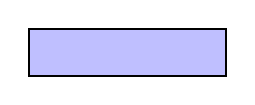
\begin{tikzpicture}[scale=1.0, transform shape]
    \tikzstyle{every node} = [draw, shape = rectangle, node distance=0mm, minimum width=4mm, minimum height=6mm, fill=blue!25!white]
    \node[draw=black, thick, minimum width=25mm] (channel1) {};
\end{tikzpicture}
}; % [label=below:{\tiny dedicated control channel}]
\end{tikzpicture}
\only<1>{\caption{\(n\) Primary users}}
\only<2>{\caption{\(n\) Spectrum channels}}
\only<3>{\caption{\(m\) Secondary users, each with at-least two radios}}
\only<4>{\caption{\textcolor{blue!75!white}{Dedicated control channel using a dedicated radio}}}
\end{center}
\end{figure}
